\section{Research Design and Methodology}
This study employs a mixed-methods approach, integrating both quantitative and qualitative research techniques to investigate the trade-offs between productivity and security in AI-assisted software development. By combining developer surveys and code security analysis, the study aims to quantify and contextualize the security risks associated with AI-generated code while assessing their impact on development efficiency.

\subsection{Hypotheses}

To systematically investigate the research questions, the study formulates the following hypotheses:

\subsubsection{For RQ1 (Perception of Trade-Offs)}

\begin{itemize}
    \item \textbf{H$_{0}$ (Null Hypothesis)}: Developers do not perceive a significant trade-off between speed and security when using AI-assisted coding tools.
    \item \textbf{H$_{1}$ (Alternative Hypothesis)}: Developers perceive a significant trade-off between speed and security when using AI-assisted coding tools.
\end{itemize}

The survey data, analyzed using descriptive statistics, correlation tests, and comparative analysis, will determine whether developers consistently report concerns about security risks in AI-assisted coding.

\subsubsection{For RQ2 (Effectiveness of Security Verification)}

\begin{itemize}
    \item \textbf{H$_{0}$ (Null Hypothesis)}: Existing security verification methods are sufficient in detecting and mitigating security vulnerabilities in AI-generated code.
    \item \textbf{H$_{1}$ (Alternative Hypothesis)}: Existing security verification methods are insufficient in detecting and mitigating security vulnerabilities in AI-generated code.
\end{itemize}

The security analysis will assess the frequency, severity, and type of vulnerabilities found in AI-generated code. Statistical evaluations, including frequency analysis and comparative benchmarking against industry security standards, will help test this hypothesis.


\subsection{Research Method}

\subsubsection{Developer Survey}

The survey will target 40-50 software developers, including 20 web developers, 5 test engineers, 5 DevOps engineers, and 10 backend developers, who actively use AI coding tools. It is designed to capture developers' perspectives on trade-offs between development speed and security risks, as well as their mitigation strategies.

Survey participants will be asked to indicate their level of agreement with various statements using a 5-point Likert scale, supplemented with open-ended questions for qualitative insights.

\paragraph{Survey Statements:}
\begin{itemize}
    \item AI tools help me write code faster, but I worry they introduce security risks.
    \item The time saved by using AI tools outweighs the effort required to fix security issues in AI-generated code.
    \item I prioritize code security over development speed when using AI tools.
    \item AI tools make it harder to follow secure coding practices (e.g., input sanitization, secure authentication).
    \item I feel pressured to deliver code quickly when using AI tools, even if it means compromising security.
\end{itemize}

\paragraph{Follow-Up Questions:}
\begin{itemize}
    \item What percentage of time saved by AI tools is spent fixing security issues?
    \item When using AI tools, how often do you review generated code for security flaws?
    \item Describe a situation where you had to choose between development speed and code security while using AI tools.
\end{itemize}

These responses will help quantify perceptions of security risks, assess common mitigation practices, and evaluate whether AI-generated efficiency gains are offset by additional security verification work.


\begin{figure}[H]
    \centering
    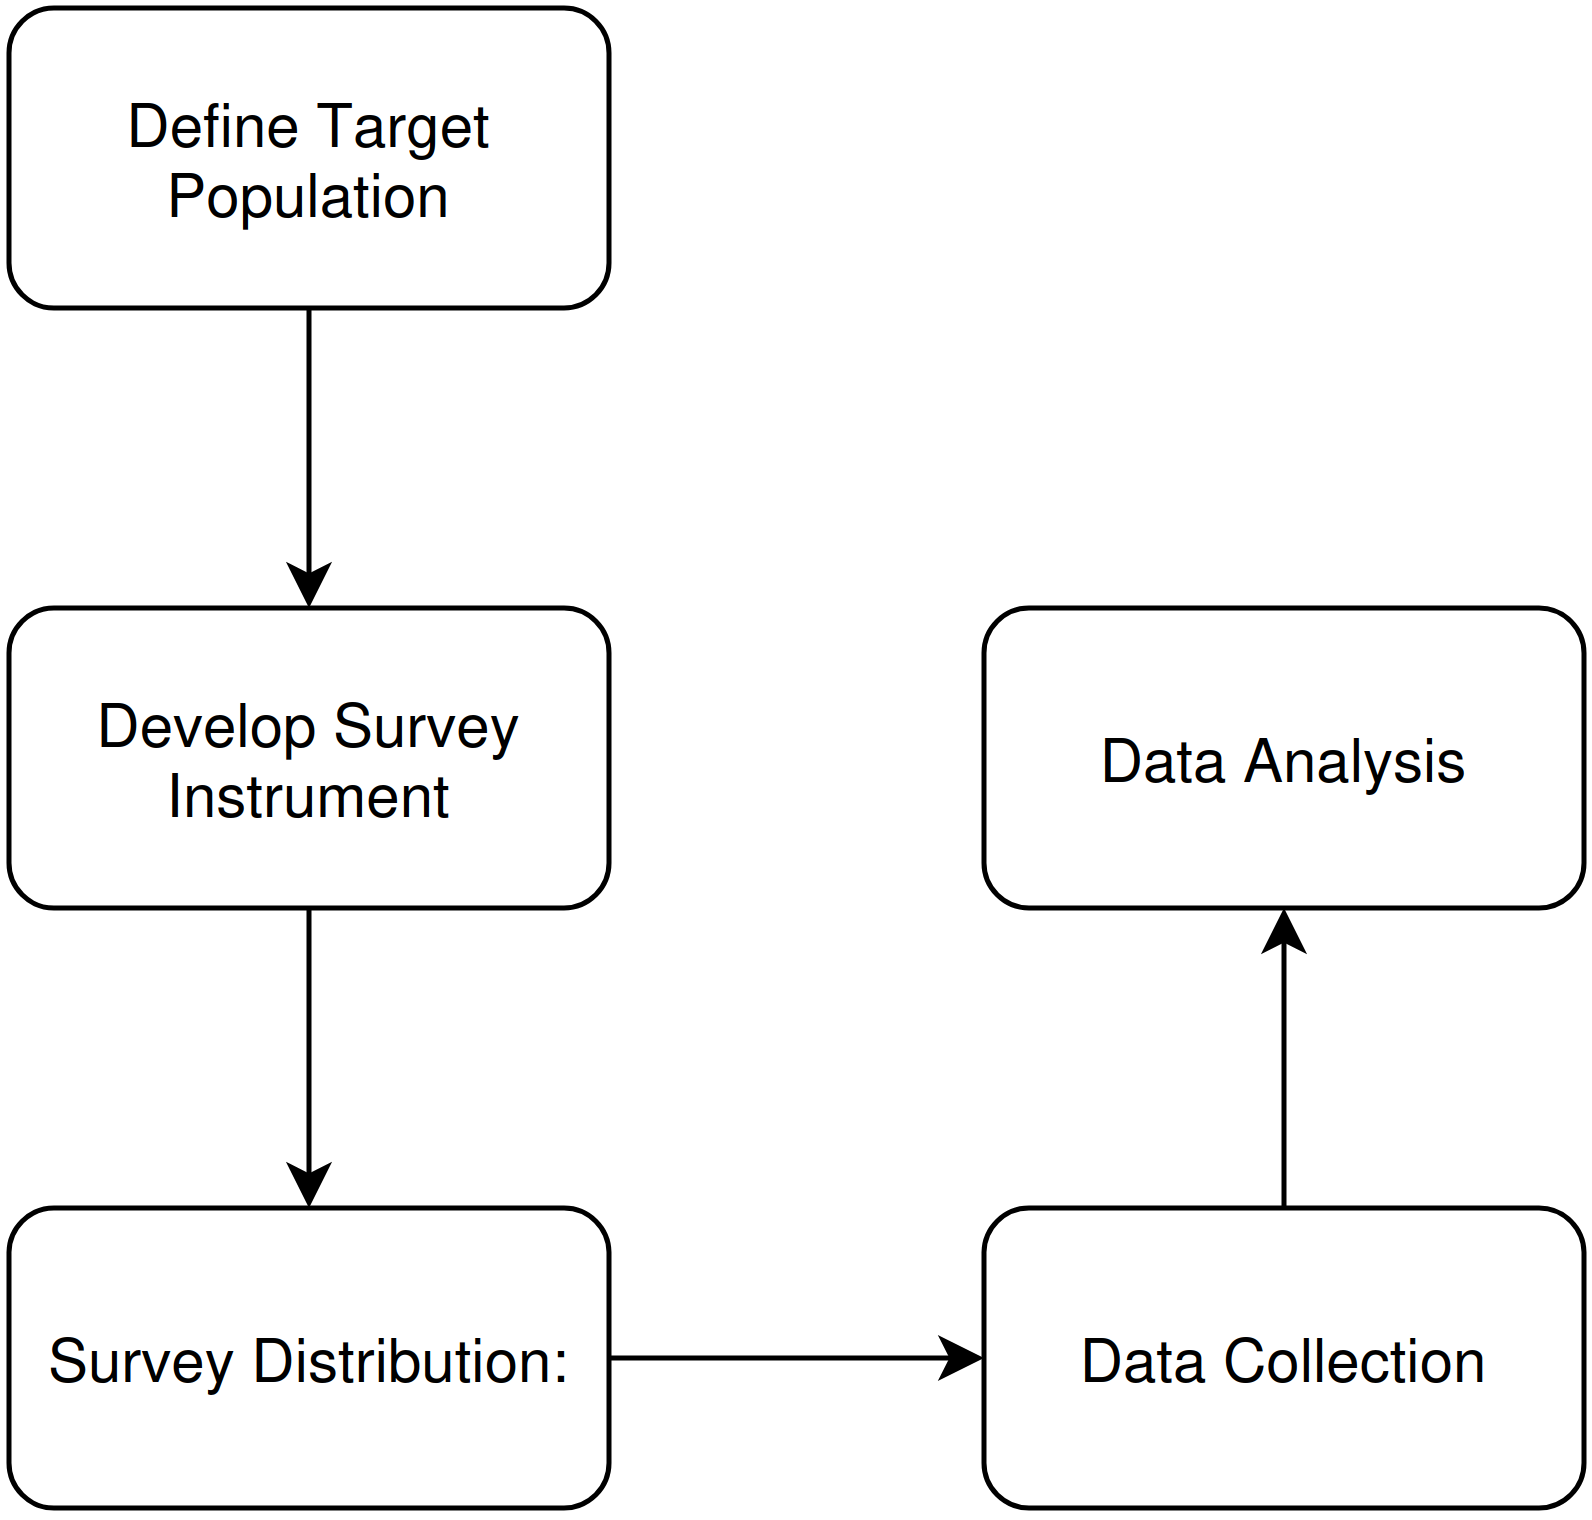
\includegraphics[width=0.9\columnwidth]{assets/survay-workflow.png}
    \caption{Workflow for the process of thesis's Developer Survey Research Method.}
    \label{fig:workflow_diagram}
\end{figure}

\subsubsection{Code Analysis}

We will compile a dataset of 25-30 AI-generated code samples by utilizing various AI coding tools and sourcing existing publicly online available examples across multiple programming languages (e.g., Python, JavaScript, Java) and use cases (e.g., web development, API security, cryptographic functions). The selected samples will represent realistic coding scenarios to facilitate an in-depth security analysis.
The methodology for security analysis includes:

\begin{itemize}
    \item \textbf{Static Analysis} – Using industry-standard tools (e.g., SonarQube, Bandit, ESLint Security Plugin) to detect potential vulnerabilities automatically.
    \item \textbf{Manual Code Review} – Conducting expert analysis of AI-generated code to identify security flaws missed by automated tools, using OWASP guidelines and secure coding principles.
    \item \textbf{Severity Classification} – Categorizing vulnerabilities based on severity (low, medium, high) and type (e.g., SQL injection, insecure authentication, hardcoded secrets).
\end{itemize}

By examining patterns in security flaws and comparing them with survey responses, this analysis provides a direct measure of security trade-offs and how developers perceive and mitigate AI-generated risks.


\begin{figure}[H]
    \centering
    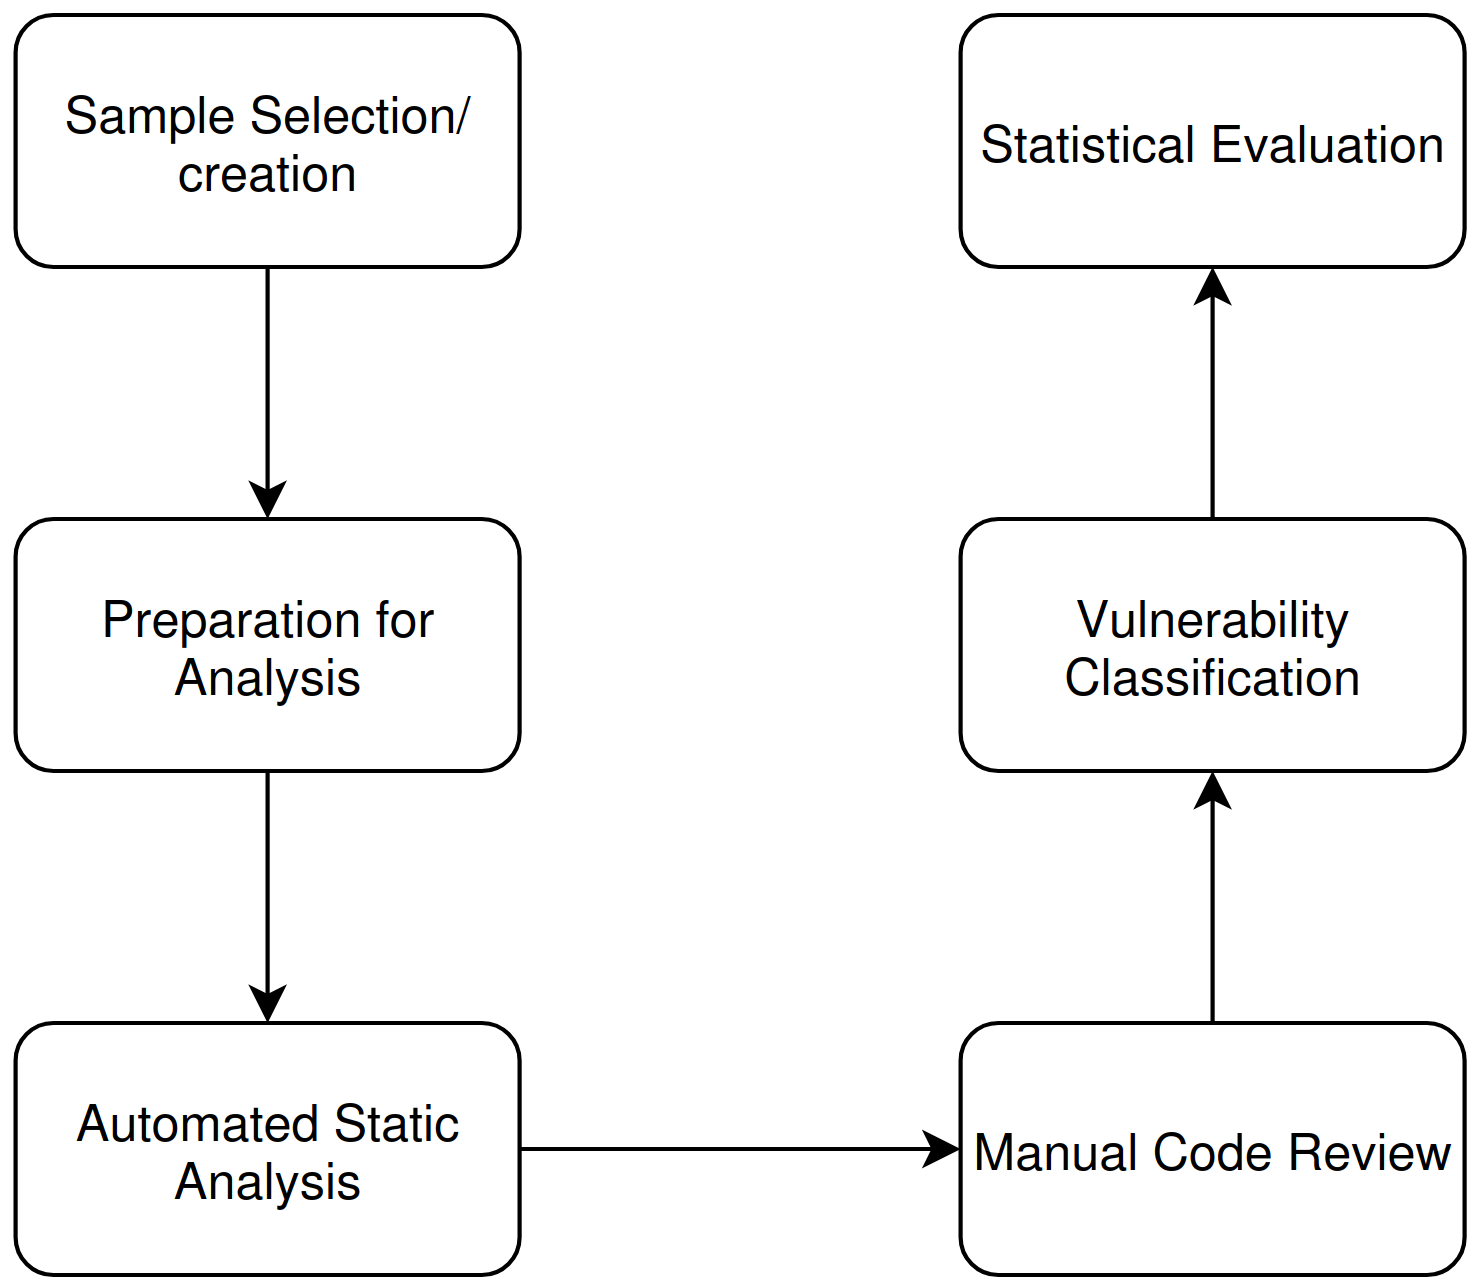
\includegraphics[width=0.9\columnwidth]{assets/data-analysis.png}
    \caption{Workflow for the process of thesis's Code Analysis Research Method.}
    \label{fig:data_analysis_diagram}
\end{figure}

\subsection{Data Analysis}

\subsubsection{Survey Data}

Survey responses will be analyzed using statistical methods, including:

\begin{itemize}
    \item \textbf{Descriptive Statistics}: Mean, median, and standard deviation will be calculated for Likert-scale responses to summarize general trends in perceptions of AI-generated code security and efficiency.
    \item \textbf{Correlation Analysis}: Pearson or Spearman correlation tests will be used to identify relationships between developers’ concerns about security risks and their reported efficiency gains.
    \item \textbf{Comparative Analysis}: Independent t-tests or ANOVA will be applied to compare responses across different groups (e.g., experience levels, programming languages used) to assess variation in perceptions.
    \item \textbf{Thematic Analysis}: Open-ended responses will be categorized using thematic coding to extract qualitative insights on developers' security concerns and mitigation strategies.
\end{itemize}

\paragraph{Motivation for Methods:} These statistical techniques allow for a robust examination of trends and relationships in the data. Descriptive statistics provide an overview of general trends, while correlation and comparative analyses help identify patterns in how different developer subgroups perceive AI tool trade-offs. Thematic analysis ensures that qualitative responses add depth to the statistical findings.

\paragraph{Addresses RQ1:} The survey data will directly reflect how developers perceive the security-efficiency trade-off, revealing trends in how security concerns impact AI tool adoption and coding behavior.

\subsubsection{Code Security Evaluation}

The identified vulnerabilities will be categorized based on severity, type, and frequency to assess the effectiveness of current security verification methods. This analysis will provide insights into whether AI-generated code introduces systematic risks and how they align with developer concerns reported in the survey.

The security analysis will include:

\begin{itemize}
    \item \textbf{Frequency Analysis}: Counting the occurrence of specific vulnerability types across AI-generated code samples.
    \item \textbf{Severity Distribution}: Categorizing vulnerabilities by severity (e.g., low, medium, high) to assess the risk posed by AI-generated code.
    \item \textbf{Comparative Evaluation}: Comparing AI-generated vulnerabilities with known industry benchmarks or previous research studies on AI-assisted coding security.
\end{itemize}

\paragraph{Motivation for Methods:} These techniques provide an empirical foundation for assessing AI-generated code security. Frequency analysis identifies recurring risks, severity classification contextualizes the impact of these vulnerabilities, and comparative evaluation allows benchmarking against existing security standards.

\paragraph{Addresses RQ2:} The security evaluation will measure the effectiveness of existing security verification methods for AI-generated code, helping to assess whether these practices are sufficient for mitigating security risks in real-world applications.

